\documentclass[t]{beamer}
\usetheme{Copenhagen}
\setbeamertemplate{headline}{} % remove toc from headers
\beamertemplatenavigationsymbolsempty

\usepackage{amsmath, array, tikz, bm, pgfplots, tcolorbox, tkz-euclide}
\usetkzobj{all}
\pgfplotsset{compat = 1.16}

\title{Measuring Angles}
\author{}
\date{}

% \begin{tcolorbox}[colframe=green!20!black, colback = green!30!white,title=\textbf{TITLE}]

\AtBeginSection[]
{
  \begin{frame}
    \frametitle{Objectives}
    \tableofcontents[currentsection]
  \end{frame}
}

\begin{document}

\begin{frame} 
\maketitle
\end{frame}

\section{Name angles and identify their parts.}

\begin{frame}{Angles}
\textbf{Angles} are formed by 2 rays with the same endpoint. \newline\\	\pause

The rays are the \textbf{sides} and the endpoint is the \textbf{vertex}.	\newline\\

\begin{center}
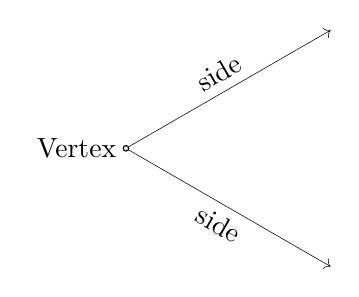
\begin{tikzpicture}
	\tkzDefPoints{0/0/A}
    \tkzDefShiftPoint[A](30:3){B}
    \tkzDefShiftPoint[A](-30:3){C}
	\tkzDrawSegments[->](A,B A,C)
	\tkzDrawPoint(A)
	\tkzLabelPoint[left](A){Vertex}
	\tkzLabelSegment[below, sloped](A,C){side}
	\tkzLabelSegment[above, sloped](A,B){side}
\end{tikzpicture}
\end{center}
\end{frame}

\begin{frame}{Naming Angles}
\begin{minipage}{0.55\textwidth}
You can name an angle by 
\begin{itemize}
    \item its vertex, $\angle A$	\newline\\
    \onslide<2->{\item a point on each ray and the vertex, $\angle BAC$ or $\angle CAB$}	\newline\\
    \onslide<3->{\item a number, $\angle 1$}
\end{itemize}
\end{minipage}
\hspace{10pt}
\begin{minipage}{0.3\textwidth}
\begin{tikzpicture}
    \tkzDefPoints{0/0/A}
    \tkzDefShiftPoint[A](30:2){B}
    \tkzDefShiftPoint[A](-30:2){C}
    \tkzDrawSegment[add = 0 and 0.5, ->, >=stealth](A,B)
    \tkzDrawSegment[add = 0 and 0.5, ->, >=stealth](A,C)
    \tkzDrawPoints(A,B,C)
    \tkzLabelPoints[left](A)
    \tkzLabelPoints[above](B)
    \tkzLabelPoints[below](C)
    \tkzLabelAngle[pos = 0.5](C,A,B){$1$}
\end{tikzpicture}
\end{minipage}
\end{frame}

\begin{frame}{Parts of an Angle}

The \textbf{interior} of an angle is the region containing all of the points between the rays.
\newline\\	\pause

The \textbf{exterior} of an angle is all of the points outside the interior.
\newline\\
\begin{center}
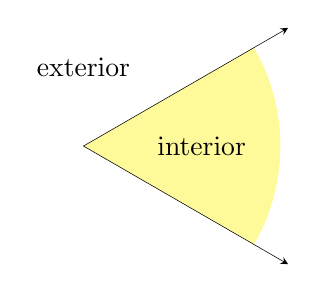
\begin{tikzpicture}
    \tkzDefPoints{0/0/A}
    \tkzDefShiftPoint[A](30:2){B}
    \tkzDefShiftPoint[A](-30:2){C}
    \path [fill=yellow!40] (30:2.5) -- (A) -- (-30:2.5) arc (-30:30:2.5);
    \tkzDrawSegment[add = 0 and 0.5, ->, >=stealth](A,B)
    \tkzDrawSegment[add = 0 and 0.5, ->, >=stealth](A,C)
    \tkzLabelAngle[pos=1.5](C,A,B){interior}
    \node at (0,1) {exterior};
\end{tikzpicture}
\end{center}
\end{frame}

\begin{frame}{Example 1}
(a)	\quad	What are two other names for $\angle 1$?
\newline\\
\begin{center}
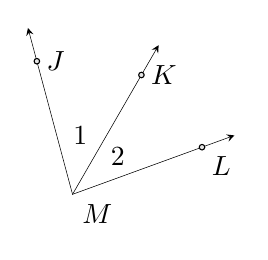
\begin{tikzpicture}
    \tkzDefPoints{0/0/M}
    \tkzDefShiftPoint[M](105:1.75){J}
    \tkzDefShiftPoint[M](60:1.75){K}
    \tkzDefShiftPoint[M](20:1.75){L}
    \tkzDrawSegments[add = 0 and 0.25, ->, >=stealth](M,J M,K M,L)
    \tkzDrawPoints(J,K,L)
    \tkzLabelPoints[right](J,K)
    \tkzLabelPoints[below right](M,L)
    \tkzLabelAngle[pos=0.75](K,M,J){1}
    \tkzLabelAngle[pos=0.75](L,M,K){2}
\end{tikzpicture}
\end{center}
\onslide<2->{\[\angle JMK \text{ and } \angle KMJ\]}
\end{frame}

\begin{frame}{Example 1}
(b)	\quad	What are two other names for $\angle KML$?
\newline\\
\begin{center}
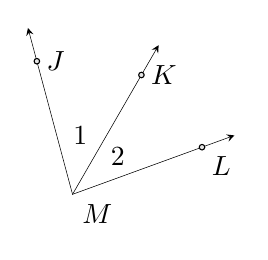
\begin{tikzpicture}
    \tkzDefPoints{0/0/M}
    \tkzDefShiftPoint[M](105:1.75){J}
    \tkzDefShiftPoint[M](60:1.75){K}
    \tkzDefShiftPoint[M](20:1.75){L}
    \tkzDrawSegments[add = 0 and 0.25, ->, >=stealth](M,J M,K M,L)
    \tkzDrawPoints(J,K,L)
    \tkzLabelPoints[right](J,K)
    \tkzLabelPoints[below right](M,L)
    \tkzLabelAngle[pos=0.75](K,M,J){1}
    \tkzLabelAngle[pos=0.75](L,M,K){2}
\end{tikzpicture}
\end{center}
\onslide<2->{\[\angle LMK \text{ and } \angle 2\]}
\end{frame}

\section{Measure angles using a protractor.}

\begin{frame}{Using a Protractor}
When measuring angles using a protractor, place the middle of the protractor at the vertex of the angle and align the $1800/0^\circ$ line along one of the angle's sides.

\onslide<2->{
\begin{center}
\begin{tikzpicture}
\tkzDefPoints{0/0/A, 4/0/B}
\tkzDefShiftPoint[A](50:4){C}
\tkzDrawSegments(A,B A,C)
\onslide<3->{\tkzProtractor[with=half,scale=0.7](A,B)}
\end{tikzpicture}
\end{center}}
\end{frame}

\begin{frame}{Example 2}
Find the measure of each angle.	\newline\\
(a)	\quad	\onslide<3->{{$\color{red}\mathbf{90^\circ}$}}
\begin{center}
\begin{tikzpicture}
	\tkzDefPoints{0/0/A, 4/0/B, 0/4/C}
	\tkzDrawSegments(A,B A,C)
	\onslide<2->{\tkzProtractor[with=half,scale=0.7](A,B)}
\end{tikzpicture}
\end{center}
\end{frame}

\begin{frame}{Example 2}
(b)	\quad	\onslide<3->{{$\color{red}\mathbf{120^\circ}$}}
\begin{center}
\begin{tikzpicture}
	\tkzDefPoints{0/0/A, 4/0/B}
	\tkzDefShiftPoint[A](120:4){C}
	\tkzDrawSegments(A,B A,C)
	\onslide<2->{\tkzProtractor[with=half,scale=0.7](A,B)}
\end{tikzpicture}
\end{center}
\end{frame}

\begin{frame}{Example 2}
(c)	\quad	\onslide<3->{{$\color{red}\mathbf{75^\circ}$}}
\begin{center}
\begin{tikzpicture}
	\tkzDefPoints{0/0/A, -4/0/B}
	\tkzDefShiftPoint[A](105:4){C}
	\tkzDrawSegments(A,B A,C)
	\onslide<2->{\tkzProtractor[with=half,scale=0.7,return](A,B)}
\end{tikzpicture}
\end{center}
\end{frame}

\section{Work with congruent angles.}

\begin{frame}{Congruent Angles}
\begin{tcolorbox}[colframe=green!20!black, colback = green!30!white,title=\textbf{Congruent Angles}]
\textbf{Congruent angles} have the same degree measure.
\end{tcolorbox}
\vspace{8pt}	\pause
\begin{center}
\begin{tikzpicture}
    \tkzDefPoints{0/0/A, 2/0/B}
    \tkzDefShiftPoint[A](40:2){C}
    \tkzDrawSegments[->, >=stealth](A,B A,C)
    \tkzLabelPoints[left](A)
    \tkzMarkAngle[size=0.5](B,A,C)
\end{tikzpicture}
\hspace{0.5in}
\begin{tikzpicture}
    \tkzDefPoints{0/0/A, 2/0/B}
    \tkzDefShiftPoint[A](40:2){C}
    \tkzDrawSegments[->, >=stealth](A,B A,C)
    %\tkzLabelPoints[left](A){$B$}
    \tkzMarkAngle[size=0.5](B,A,C)
    \tkzLabelAngle[pos=-0.25](B,A,C){$B$}
\end{tikzpicture}   
\end{center}
\begin{align*}
\onslide<3->{m\angle A &= m\angle B} \\[8pt]
\onslide<4->{\angle A &\cong \angle B}
\end{align*}
\end{frame}

\begin{frame}{Example 3}
Use the figure to find the missing value.	\newline\\
\begin{minipage}{0.35\textwidth}
    (a)	\quad $\angle JMK \cong \, ?$	\\[10pt]
    \onslide<2->{$\angle RMG$} \\[15pt]
    \onslide<3->{(b) \quad $\angle IGN \cong \, ?$}	\\[10pt]
    \onslide<4->{$\angle HGM$} \\[15pt]
    \onslide<5->{(c) \quad $\angle RMP \cong \, ?$}	\\[10pt]
    \onslide<6->{$\angle QHL$}
\end{minipage}
\begin{minipage}{0.60\textwidth}
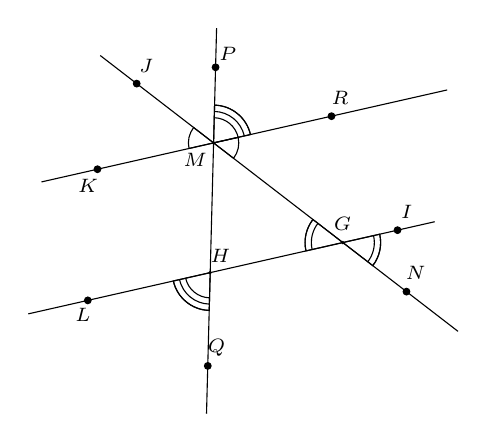
\begin{tikzpicture}[scale=0.8]
\draw [shift={(0.9524041328051618,3.159458079797444)}] (0,0) -- (142.3675785601059:0.4) arc (142.3675785601059:192.77349910381227:0.4) -- cycle;
\draw [shift={(0.9524041328051618,3.159458079797444)}] (0,0) -- (-37.63242143989409:0.4) arc (-37.63242143989409:12.773499103812204:0.4) -- cycle;
\draw [shift={(0.9524041328051618,3.159458079797444)}] (0,0) -- (12.773499103812197:0.6) arc (12.773499103812197:88.50241226098248:0.6) -- cycle;
\draw [shift={(0.8985630736392743,1.100037566702241)}] (0,0) -- (-167.2265008961878:0.6) arc (-167.2265008961878:-91.49758773901755:0.6) -- cycle;
\draw [shift={(3.0043099408008302,1.57742738441278)}] (0,0) -- (-37.63242143989412:0.6) arc (-37.63242143989412:12.773499103812243:0.6) -- cycle;
\draw [shift={(3.0043099408008302,1.57742738441278)}] (0,0) -- (142.36757856010593:0.6) arc (142.36757856010593:192.7734991038122:0.6) -- cycle;
\draw (1.,4.98)-- (0.84,-1.14);
\draw (-1.78,2.54)-- (4.66,4.);
\draw (-1.9902301599211032,0.44512481499445367)-- (4.462707379638399,1.9080578596771978);
\draw (-0.8468806902748067,4.546716602464624)-- (4.832413823626125,0.1679492077285536);
\draw [shift={(0.9524041328051618,3.159458079797444)}] (12.773499103812197:0.6) arc (12.773499103812197:88.50241226098248:0.6);
\draw [shift={(0.9524041328051618,3.159458079797444)}] (12.773499103812197:0.5) arc (12.773499103812197:88.50241226098248:0.5);
\draw [shift={(0.9524041328051618,3.159458079797444)}] (12.773499103812197:0.4) arc (12.773499103812197:88.50241226098248:0.4);
\draw [shift={(0.8985630736392743,1.100037566702241)}] (-167.2265008961878:0.6) arc (-167.2265008961878:-91.49758773901755:0.6);
\draw [shift={(0.8985630736392743,1.100037566702241)}] (-167.2265008961878:0.5) arc (-167.2265008961878:-91.49758773901755:0.5);
\draw [shift={(0.8985630736392743,1.100037566702241)}] (-167.2265008961878:0.4) arc (-167.2265008961878:-91.49758773901755:0.4);
\draw [shift={(3.0043099408008302,1.57742738441278)}] (-37.63242143989412:0.6) arc (-37.63242143989412:12.773499103812243:0.6);
\draw [shift={(3.0043099408008302,1.57742738441278)}] (-37.63242143989412:0.5) arc (-37.63242143989412:12.773499103812243:0.5);
\draw [shift={(3.0043099408008302,1.57742738441278)}] (142.36757856010593:0.6) arc (142.36757856010593:192.7734991038122:0.6);
\draw [shift={(3.0043099408008302,1.57742738441278)}] (142.36757856010593:0.5) arc (142.36757856010593:192.7734991038122:0.5);
\begin{scriptsize}
\draw [fill=black] (0.9837882604055497,4.359900960512274) circle (1.5pt);
\draw[color=black] (1.18,4.57) node {$P$};
\draw [fill=black] (2.8236964398741433,3.583695155623641) circle (1.5pt);
\draw[color=black] (2.96,3.87) node {$R$};
\draw [fill=black] (3.8722475262264204,1.7741958432204452) circle (1.5pt);
\draw[color=black] (4.02,2.07) node {$I$};
\draw [fill=black] (4.014383302021494,0.7986552517862973) circle (1.5pt);
\draw[color=black] (4.16,1.09) node {$N$};
\draw [fill=black] (0.8598557097118462,-0.3805191035218787) circle (1.5pt);
\draw[color=black] (1.,-0.09) node {$Q$};
\draw [fill=black] (-1.044431035046088,0.6595451134909633) circle (1.5pt);
\draw[color=black] (-1.12,0.43) node {$L$};
\draw [fill=black] (-0.891267830442241,2.7414827589370074) circle (1.5pt);
\draw[color=black] (-1.04,2.47) node {$K$};
\draw [fill=black] (-0.26853570513602965,4.1008094290232275) circle (1.5pt);
\draw[color=black] (-0.12,4.39) node {$J$};
\draw [fill=black] (0.9524041328051618,3.159458079797444) circle (0.5pt);
\draw[color=black] (0.66,2.89) node {$M$};
\draw [fill=black] (0.8985630736392743,1.100037566702241) circle (0.5pt);
\draw[color=black] (1.06,1.37) node {$H$};
\draw [fill=black] (3.0043099408008302,1.57742738441278) circle (0.5pt);
\draw[color=black] (3.,1.87) node {$G$};
\end{scriptsize}
\end{tikzpicture}
\end{minipage}
\end{frame}

\section{Solve problems using the Angle Addition Postulate}

\begin{frame}{Angle Addition Postulate}
The \textbf{Angle Addition Postulate} is similar to the Segment Addition Postulate.	\newline\\	\pause

If $B$ is in the interior of $\angle AOC$ then \[m\angle AOB + m\angle BOC = m\angle AOC\]	\vspace{4pt}
\begin{center}
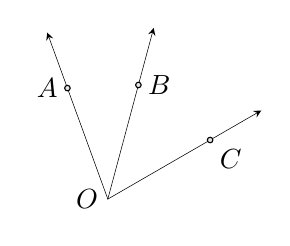
\begin{tikzpicture}
    \tkzDefPoints{0/0/O}
    \tkzDefShiftPoint[O](110:1.5){A}
    \tkzDefShiftPoint[O](75:1.5){B}
    \tkzDefShiftPoint[O](30:1.5){C}
    \tkzDrawSegments[add = 0 and 0.5, ->, >=stealth](O,A O,B O,C)
    \tkzDrawPoints(A,B,C)
    \tkzLabelPoints[left](A,O)
    \tkzLabelPoints[right](B)
    \tkzLabelPoints[below right](C)
\end{tikzpicture}
\end{center}
\end{frame}

\begin{frame}{Example 4}
Find the measure of each angle.	\newline\\
(a)	\quad $m\angle LKN = 145^\circ$	\newline\\
\begin{minipage}{0.4\textwidth}
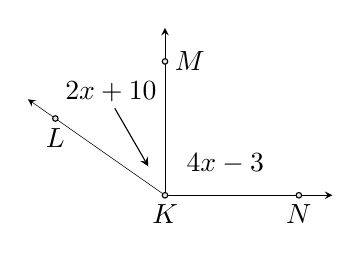
\begin{tikzpicture}[scale=0.85]
    \tkzDefPoints{0/0/K, 2/0/N}
    \tkzDefShiftPoint[K](90:2){M}
    \tkzDefShiftPoint[K](145:2){L}
    \tkzDrawSegments[add = 0 and 0.25, ->, >=stealth](K,N K,M K,L)
    \tkzDrawPoints(K,L,M,N)
    \tkzLabelPoints[below](L,K,N)
    \tkzLabelPoints[right](M)
    \tkzLabelAngle[pos=0.25, above right](N,K,M){$4x-3$}
    \tkzLabelAngle[pos=1.75](M,K,L){$2x+10$}
    \draw [->, >=stealth](120:1.5) -- (120:0.5);
\end{tikzpicture}
\end{minipage}
\begin{minipage}{0.55\textwidth}
\begin{align*}
\onslide<2->{m\angle LKM + m\angle MKN &= m\angle LKN}	\\
\onslide<3->{2x+10 + 4x-3 &= 145} \\
\onslide<4->{6x+7 &= 145} \\
\onslide<5->{6x &= 138} \\
\onslide<6->{x &= 23}
\end{align*}
\end{minipage}
\begin{align*}
\onslide<7->{m\angle LKM &= 2(23)+10 & m\angle MKN &= 4(23)-3}	\\
\onslide<8->{m\angle LKM &= 56^\circ & m\angle MKN &= 89^\circ}
\end{align*}
\end{frame}

\begin{frame}{Example 4}
(b)	\quad Given $\overleftrightarrow{KM}$	\newline\\
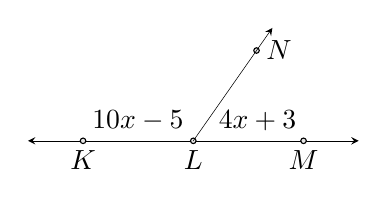
\begin{tikzpicture}[scale=0.8]
    \tkzDefPoints{0/0/L, 1.75/0/M, -1.75/0/K}
    \tkzDefShiftPoint[L](55:1.75){N}
    \tkzDrawSegment[add = 0.25 and 0.25, <->, >=stealth](K,M)
    \tkzLabelPoints[below](K,L,M)
    \tkzDrawPoints(K,L,M,N)
    \tkzLabelPoints[right](N)
    \tkzDrawSegment[add = 0 and 0.25, ->, >=stealth](L,N)
    \node at (0,0) [anchor = south east] {$10x-5$};
    \node at (0.25,0) [anchor = south west] {$4x+3$};
\end{tikzpicture}
\end{frame}

\end{document}